\documentclass[11pt]{article}
\usepackage[margin=0.9in]{geometry}
\usepackage{booktabs}
\usepackage{graphicx}
\usepackage{pdflscape}
\begin{document}
\section*{Weighted 2+2 cross-scaling boundary}
\texttt{projective-law-cross-scale22/v1}. The source checker compares eight
power intermediates, eight cross-scaled inputs, and seven composed coefficient
expressions from Rust and Lean as expanded integer polynomials. All 23 match.
Multiplication-to-addition mutations on both sides and a composed-coefficient
subtraction mutation are rejected.

\begin{center}
\begin{tabular}{lccc}
\toprule
Input & Common $Z$ power & Common $W$ power & Equal\\
\midrule
q1c & 2 & 0 & yes\\
q2c & 2 & 0 & yes\\
r1c & 4 & 0 & yes\\
r2c & 4 & 0 & yes\\
s1c & 3 & 1 & yes\\
s2c & 3 & 1 & yes\\
t1c & 5 & 1 & yes\\
t2c & 5 & 1 & yes\\
\bottomrule
\end{tabular}
\end{center}
\noindent The Lean theorem proves these common weights from the weighted
numerator equations over a commutative ring. Five further theorems derive
$B=Z^8B_{aff}$, $A=Z^9WA_{aff}$, and $C=Z^7WC_{aff}$, plus nonzero
$B,C$ equivalence when $Z,W$ are nonzero. It does not establish the
returned Jacobian class, exceptional branches, or a cost change. The
accompanying CSV and JSON retain all 23 rows and all polynomial terms.
\clearpage
\begin{landscape}
\section*{Input and coefficient weights}
\begin{center}
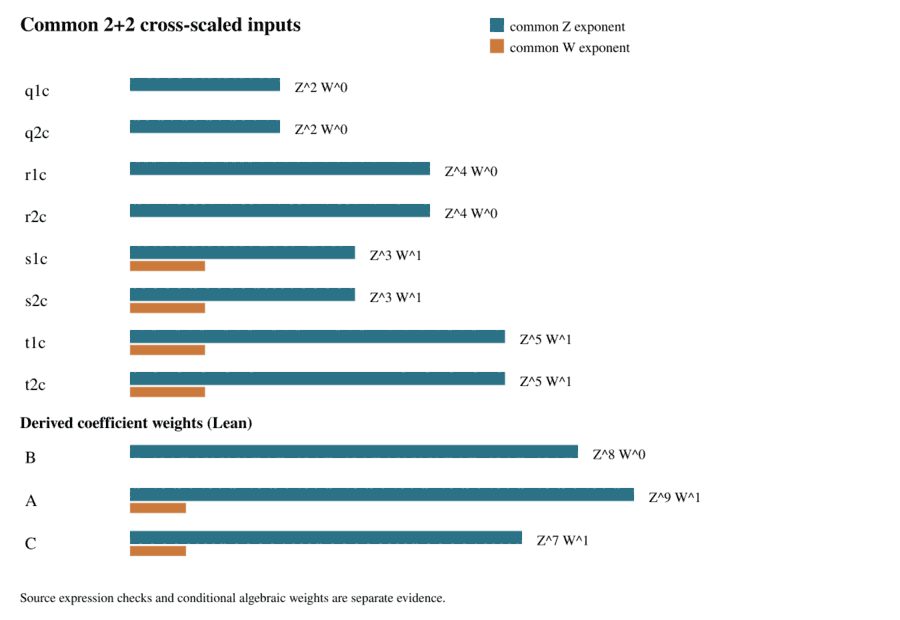
\includegraphics[width=0.94\linewidth]{cross-scale22.png}
\end{center}
\end{landscape}
\end{document}
